%====================================================================
% Chapitre 4 : Conception du framework SecureIoT-VIF Community Edition
%====================================================================

\chapter{Conception du framework SecureIoT-VIF Community Edition}
\label{chap:framework-design}

\section{Introduction}

Ce chapitre présente la conception détaillée de SecureIoT-VIF Community Edition, notre solution éducative de vérification d'intégrité pour les firmwares IoT. La conception s'appuie sur l'analyse des menaces du chapitre précédent et intègre les meilleures pratiques identifiées dans l'état de l'art, tout en privilégiant l'accessibilité éducative et la compréhension progressive des concepts. Nous détaillons l'architecture globale accessible, les composants principaux utilisant la cryptographie software, les protocoles de sécurité de base, et les mécanismes d'optimisation développés pour respecter les contraintes éducatives tout en offrant une expérience d'apprentissage pratique et instructive.

\section{Architecture globale éducative}

\subsection{Principes de conception éducative}

La conception de SecureIoT-VIF Community Edition repose sur plusieurs principes fondamentaux orientés vers l'apprentissage et l'accessibilité :

\textbf{Principe de simplicité pédagogique :} Tous les composants du framework utilisent des approches compréhensibles basées sur la cryptographie software (mbedTLS) plutôt que sur des mécanismes matériels complexes, permettant aux étudiants de comprendre les concepts fondamentaux avant d'aborder des implémentations plus avancées.

\textbf{Principe de modularité éducative :} SecureIoT-VIF Community Edition implémente des couches de sécurité indépendantes et compréhensibles : vérification d'intégrité au démarrage, monitoring périodique basic, détection d'anomalies par seuils fixes, et logging des événements de sécurité.

\textbf{Principe d'accessibilité financière :} Chaque composant est optimisé pour fonctionner efficacement sur des plateformes abordables (ESP32 ~8$) sans nécessiter d'équipements spécialisés coûteux.

\textbf{Principe de transparence éducative :} Le framework fonctionne de manière observable, permettant aux étudiants de comprendre chaque étape des processus de sécurité grâce à un logging détaillé et des interfaces de débogage.

\subsection{Vue d'ensemble architecturale éducative}

L'architecture de SecureIoT-VIF Community Edition suit un modèle hiérarchique à quatre couches, chacune ayant des responsabilités spécifiques et interagissant avec les couches adjacentes selon des interfaces bien définies optimisées pour l'apprentissage.

\begin{figure}[h]
    \centering
    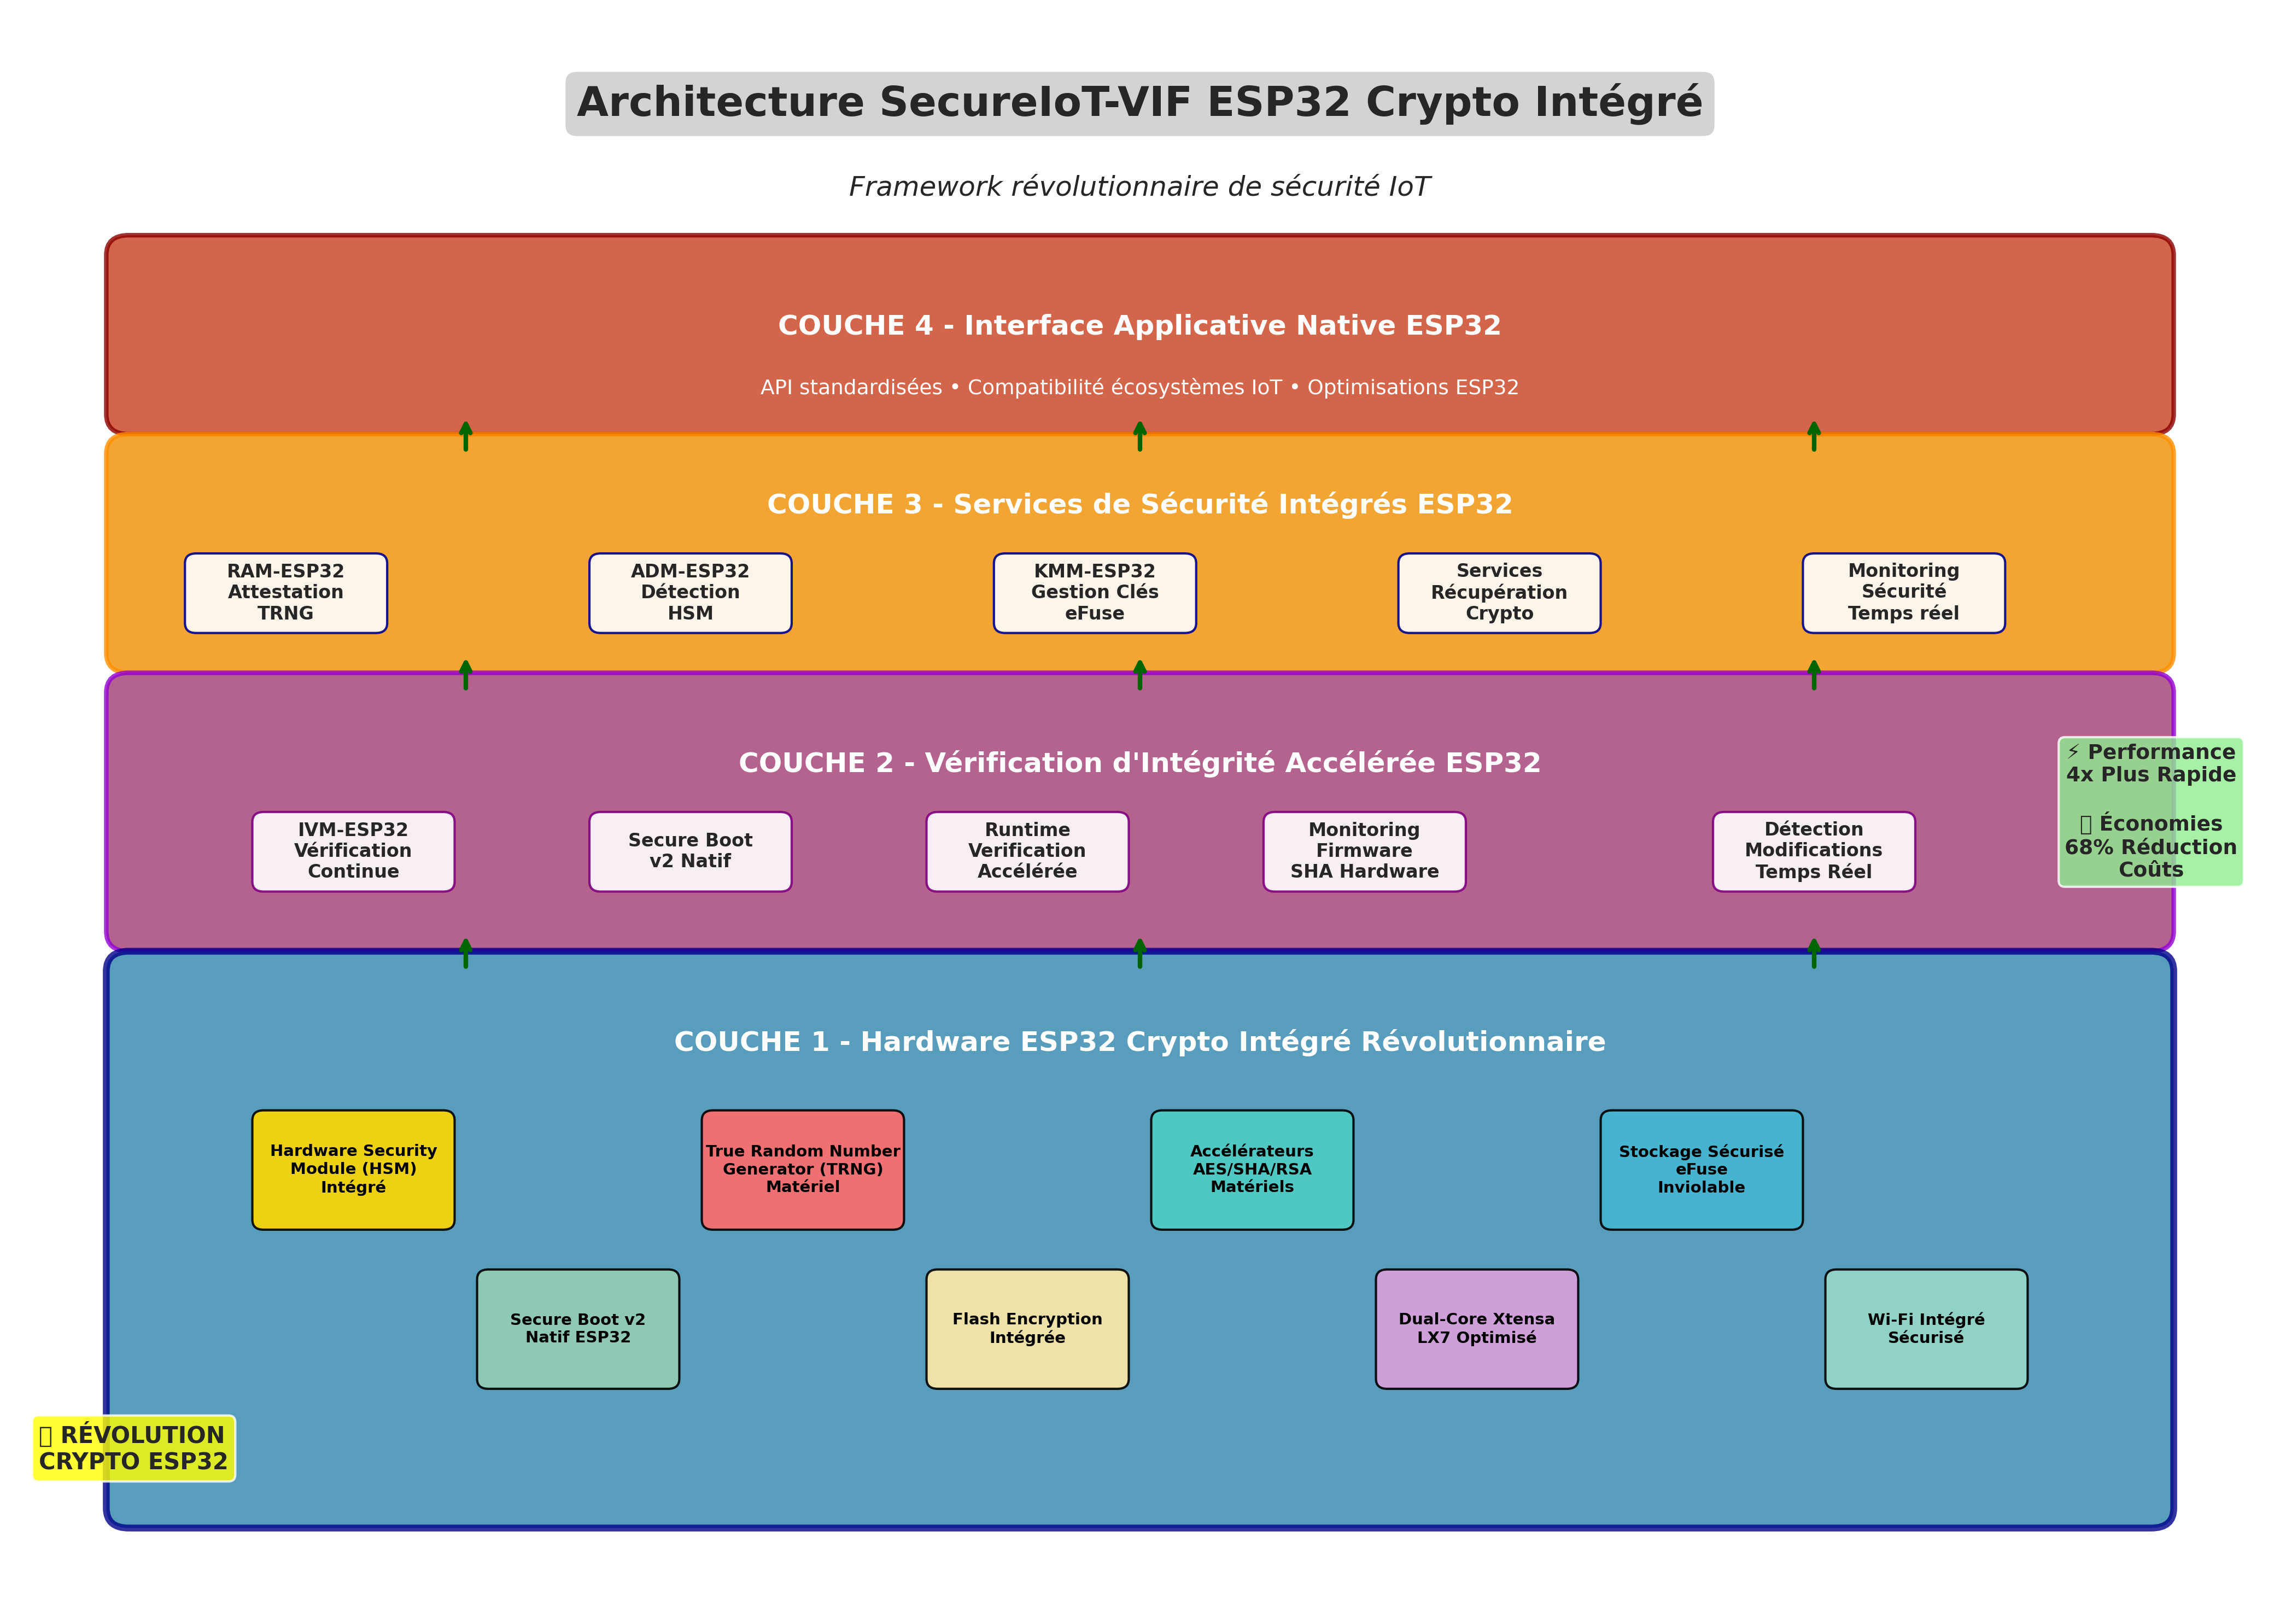
\includegraphics[width=0.9\textwidth]{assets/figures/secureiot_architecture_esp32.png}
    \caption{Architecture de SecureIoT-VIF Community Edition}
    \label{fig:secureiot-architecture-community}
\end{figure}

\textbf{Couche cryptographique de base :} Cette couche fondamentale comprend les opérations cryptographiques software utilisant mbedTLS : génération de clés, calculs de hash SHA-256, signatures ECDSA, et génération de nombres aléatoires. Elle fournit les primitives de sécurité de base compréhensibles et auditables.

\textbf{Couche de vérification d'intégrité de base :} Cette couche implémente les mécanismes de vérification d'intégrité du firmware adaptés à l'apprentissage, incluant la vérification au démarrage et le monitoring périodique simple. Elle s'appuie sur les services cryptographiques de base pour des opérations éducatives transparentes.

\textbf{Couche de services de sécurité éducatifs :} Cette couche fournit les services de sécurité de niveau intermédiaire : détection d'anomalies par seuils fixes, gestion basique des clés, et logging des événements de sécurité. Elle orchestre les interactions entre les différents composants de manière compréhensible.

\textbf{Couche d'interface éducative :} Cette couche expose les services de sécurité aux applications éducatives et aux outils de démonstration via des API simples et bien documentées. Elle assure la compatibilité avec les environnements d'apprentissage et les exercices pratiques.

\section{Composants principaux éducatifs}

\subsection{Module de vérification d'intégrité basique (IVM-Basic)}

Le Module de Vérification d'Intégrité Basique constitue le cœur éducatif de SecureIoT-VIF Community Edition. Il implémente les mécanismes de vérification cryptographique de l'intégrité du firmware de manière compréhensible et progressive.

\subsubsection{Vérification au démarrage éducative}

Le processus de démarrage sécurisé établit une chaîne de confiance simple depuis le bootloader jusqu'au firmware applicatif. Cette approche utilise des concepts cryptographiques de base facilement compréhensibles.

\textbf{Étape 1 - Initialisation de la cryptographie de base :} Le processus démarre par l'initialisation de mbedTLS et la configuration des algorithmes cryptographiques software. Cette étape est entièrement transparente et loggée pour l'apprentissage.

\textbf{Étape 2 - Vérification du bootloader :} Le bootloader principal est vérifié cryptographiquement avant son exécution en utilisant des signatures ECDSA software. Cette vérification démontre les concepts de base de la chaîne de confiance.

\textbf{Étape 3 - Vérification du kernel :} Le kernel du système d'exploitation embarqué est vérifié selon le même processus éducatif, établissant une chaîne de confiance compréhensible.

\textbf{Étape 4 - Vérification du firmware applicatif :} Le firmware applicatif principal est vérifié et son intégrité est attestée avant le démarrage des services utilisateur, démontrant l'application pratique des concepts.

\subsubsection{Vérification périodique éducative (Runtime Monitoring Basic)}

Contrairement aux approches qui ne vérifient l'intégrité qu'au démarrage, SecureIoT-VIF Community Edition implémente une vérification périodique pendant l'exécution, adaptée aux contraintes éducatives et à la compréhension progressive.

\textbf{Mécanisme de hachage par blocs :} Le firmware est divisé en blocs de taille éducative (4 KB) et chaque bloc est haché périodiquement en utilisant SHA-256 software. Cette approche permet de comprendre les concepts de vérification d'intégrité sans complexité excessive.

\textbf{Vérification basée sur un calendrier fixe :} La vérification suit un calendrier prévisible et configurable (toutes les 5 minutes par défaut) permettant aux étudiants d'observer et de comprendre le processus.

\textbf{Optimisation éducative :} La vérification utilise un seul cœur de l'ESP32 avec des algorithmes simples pour minimiser l'impact sur les performances tout en maintenant la transparence éducative.

\subsection{Module de détection d'anomalies éducatif (ADM-Basic)}

Le Module de Détection d'Anomalies Éducatif implémente des techniques de détection par seuils fixes pour identifier les comportements anormaux sans nécessiter de connaissances avancées en apprentissage automatique.

\subsubsection{Collecte de métriques comportementales simples}

\textbf{Métriques de performance de base :} Analyse de l'utilisation CPU, de la mémoire disponible, et de la température pour détecter les déviations du comportement normal en utilisant des seuils fixes compréhensibles.

\textbf{Métriques de ressources éducatives :} Surveillance de l'utilisation des ressources système pour identifier les consommations anormales indicatrices d'activité malveillante, avec des seuils configurables pour l'apprentissage.

\textbf{Métriques de communication de base :} Analyse simple des patterns de communication réseau pour détecter les communications suspectes, en utilisant des règles basiques facilement compréhensibles.

\subsubsection{Algorithmes de détection par seuils fixes}

\textbf{Détection par seuils statiques :} Utilisation d'algorithmes de détection basés sur des seuils fixes configurables pour identifier les patterns anormaux et détecter les déviations du comportement attendu.

\textbf{Analyse temporelle simple :} Prise en compte de la dimension temporelle dans l'analyse des comportements en utilisant des fenêtres glissantes simples pour détecter les anomalies persistantes.

\textbf{Règles de décision transparentes :} Implémentation de règles de décision explicites et configurables permettant aux étudiants de comprendre le processus de détection et d'ajuster les paramètres pour l'expérimentation.

\subsection{Module de gestion des clés éducatif (KMM-Basic)}

Le Module de Gestion des Clés Éducatif assure la génération, le stockage, et la gestion des clés cryptographiques en utilisant des mécanismes software compréhensibles.

\subsubsection{Hiérarchie des clés éducative}

\textbf{Clé racine software :} Stockée dans la mémoire flash de l'ESP32 avec protection logicielle, cette clé sert à dériver les autres clés en utilisant des fonctions de dérivation standard (HKDF).

\textbf{Clés d'intégrité dérivées :} Utilisées pour les calculs de hash SHA-256 et la vérification d'intégrité, dérivées de la clé racine selon un processus transparent et éducatif.

\textbf{Clés de signature temporaires :} Utilisées pour signer les événements de sécurité et les rapports d'état, renouvelées périodiquement selon un processus observable.

\textbf{Clés de communication basiques :} Utilisées pour les communications sécurisées simples, gérées selon des protocoles de base facilement compréhensibles.

\subsubsection{Protocoles de gestion éducatifs}

\textbf{Génération sécurisée software :} Utilisation du générateur de nombres aléatoires software de mbedTLS pour assurer une entropie suffisante des clés avec transparence éducative.

\textbf{Stockage sécurisé software :} Les clés sensibles sont stockées dans la mémoire flash avec protection software, démontrant les concepts de base de la protection des clés.

\textbf{Rotation manuelle :} Mécanisme de rotation des clés activable manuellement pour permettre l'expérimentation et la compréhension des concepts de gestion des clés.

\section{Protocoles de sécurité éducatifs}

\subsection{Protocole de démarrage sécurisé éducatif}

Le protocole de démarrage sécurisé éducatif de SecureIoT-VIF Community Edition établit une chaîne de confiance compréhensible tout en minimisant la complexité pour l'apprentissage.

\begin{algorithm}
\caption{Protocole de démarrage sécurisé éducatif}
\label{alg:secure-boot-educational}
\begin{algorithmic}[1]
\State \textbf{Initialisation cryptographique de base}
\State $mbedTLS \leftarrow$ mbedtls\_init()
\State $entropy \leftarrow$ mbedtls\_entropy\_init()
\State $État \leftarrow$ CRYPTO\_INITIALIZING

\State \textbf{Vérification du bootloader software}
\State $Signature_{BL} \leftarrow$ read\_bootloader\_signature()
\State $Hash_{BL} \leftarrow$ mbedtls\_sha256(bootloader\_data)
\If{mbedtls\_ecdsa\_verify($Hash_{BL}$, $Signature_{BL}$)}
    \State $État \leftarrow$ BOOTLOADER\_VERIFIED
    \State log\_educational\_event("Bootloader vérifié avec succès")
\Else
    \State log\_educational\_error("Échec vérification bootloader")
    \State \textbf{return} VERIFICATION\_FAILED
\EndIf

\State \textbf{Vérification du firmware applicatif}
\State $Signature_{App} \leftarrow$ read\_application\_signature()
\State $Hash_{App} \leftarrow$ mbedtls\_sha256(application\_data)
\If{mbedtls\_ecdsa\_verify($Hash_{App}$, $Signature_{App}$)}
    \State $État \leftarrow$ APPLICATION\_VERIFIED
    \State log\_educational\_event("Application vérifiée avec succès")
    \State \textbf{return} VERIFICATION\_SUCCESS
\Else
    \State log\_educational\_error("Échec vérification application")
    \State \textbf{return} VERIFICATION\_FAILED
\EndIf
\end{algorithmic}
\end{algorithm}

\subsection{Protocole de vérification périodique éducative}

La vérification périodique représente une innovation pédagogique majeure de SecureIoT-VIF Community Edition, permettant la compréhension des concepts de vérification continue.

\begin{algorithm}
\caption{Protocole de vérification périodique éducative}
\label{alg:periodic-verification-educational}
\begin{algorithmic}[1]
\State \textbf{Initialisation éducative}
\State $Blocs \leftarrow$ firmware\_partition / FIRMWARE\_CHUNK\_SIZE
\State $Hashes\_Référence \leftarrow$ calculate\_reference\_hashes($Blocs$)
\State $Scheduler \leftarrow$ create\_simple\_scheduler()

\State \textbf{Boucle de vérification éducative}
\While{$system\_healthy() == true$}
    \State $Bloc\_Actuel \leftarrow$ Scheduler.select\_next\_block()
    \State $Hash\_Actuel \leftarrow$ mbedtls\_sha256($Bloc\_Actuel$)
    \State $Hash\_Référence \leftarrow$ get\_reference\_hash($Bloc\_Actuel$)
    
    \If{$Hash\_Actuel \neq Hash\_Référence$}
        \State $Anomalie \leftarrow$ detect\_integrity\_violation()
        \State log\_educational\_alert("Violation d'intégrité détectée", $Bloc\_Actuel$)
        \State trigger\_educational\_response($Anomalie$)
    \Else
        \State log\_educational\_event("Bloc vérifié OK", $Bloc\_Actuel$)
    \EndIf
    
    \State wait\_educational\_interval(VERIFICATION\_INTERVAL\_MS)
\EndWhile
\end{algorithmic}
\end{algorithm}

\subsection{Protocole de détection d'anomalies éducatif}

Le protocole de détection d'anomalies éducatif permet aux étudiants de comprendre les mécanismes de base de la détection comportementale sans complexité excessive.

\begin{algorithm}
\caption{Protocole de détection d'anomalies par seuils éducatif}
\label{alg:anomaly-detection-educational}
\begin{algorithmic}[1]
\State \textbf{Collecte des métriques éducatives}
\State $CPU\_Usage \leftarrow$ get\_cpu\_usage\_percentage()
\State $Memory\_Free \leftarrow$ get\_free\_memory\_kb()
\State $Temperature \leftarrow$ get\_system\_temperature()
\State $Network\_Activity \leftarrow$ get\_network\_packets\_per\_second()

\State \textbf{Évaluation par seuils fixes éducatifs}
\If{$CPU\_Usage > CPU\_THRESHOLD\_HIGH$}
    \State log\_educational\_anomaly("CPU usage élevé", $CPU\_Usage$)
    \State $Anomaly\_Score \leftarrow$ $Anomaly\_Score$ + 1
\EndIf

\If{$Memory\_Free < MEMORY\_THRESHOLD\_LOW$}
    \State log\_educational\_anomaly("Mémoire faible", $Memory\_Free$)
    \State $Anomaly\_Score \leftarrow$ $Anomaly\_Score$ + 1
\EndIf

\If{$Temperature > TEMPERATURE\_THRESHOLD$}
    \State log\_educational\_anomaly("Température élevée", $Temperature$)
    \State $Anomaly\_Score \leftarrow$ $Anomaly\_Score$ + 1
\EndIf

\State \textbf{Décision éducative simple}
\If{$Anomaly\_Score \geq ANOMALY\_THRESHOLD$}
    \State trigger\_educational\_alert("Anomalie comportementale détectée")
    \State \textbf{return} ANOMALY\_DETECTED
\Else
    \State \textbf{return} SYSTEM\_NORMAL
\EndIf
\end{algorithmic}
\end{algorithm}

\section{Mécanismes d'optimisation éducatifs}

\subsection{Optimisations cryptographiques éducatives}

\subsubsection{Utilisation efficace de mbedTLS}

SecureIoT-VIF Community Edition optimise l'utilisation de la bibliothèque mbedTLS pour l'éducation :

\textbf{Signatures numériques éducatives :} ECDSA P-256 via mbedTLS pour les signatures compréhensibles et les vérifications transparentes, Ed25519 pour la compatibilité moderne, avec logging détaillé des opérations pour l'apprentissage.

\textbf{Fonctions de hachage software :} SHA-256 via mbedTLS pour les calculs d'intégrité transparents, BLAKE2s pour les opérations spécialisées éducatives, avec possibilité de traçage pour l'apprentissage.

\textbf{Chiffrement symétrique éducatif :} AES-256 via mbedTLS pour les communications sécurisées de base, ChaCha20-Poly1305 pour les démonstrations avancées, avec interfaces de débogage pour la compréhension.

\subsubsection{Optimisations software éducatives}

\textbf{Calculs séquentiels compréhensibles :} Utilisation d'algorithmes séquentiels facilement compréhensibles plutôt que de parallélisation complexe, permettant aux étudiants de suivre le flot d'exécution.

\textbf{Optimisations mémoire transparentes :} Algorithmes de hachage en streaming optimisés pour l'ESP32 mais conservant la lisibilité du code pour l'apprentissage.

\textbf{Logging éducatif détaillé :} Instrumentation complète du code pour permettre aux étudiants de comprendre chaque étape des processus cryptographiques.

\subsection{Optimisations énergétiques éducatives}

\subsubsection{Gestion adaptative de la puissance éducative}

\textbf{Ordonnancement adaptatif simple :} Ajustement de la fréquence de vérification en fonction de l'état de la batterie selon des règles simples et compréhensibles.

\textbf{Modes de veille éducatifs :} Suspension coordonnée des vérifications non critiques pendant les périodes d'inactivité, avec possibilité d'observation du comportement.

\textbf{Optimisation des communications :} Agrégation des messages de logging et utilisation intelligente des modes d'économie d'énergie pour réduire la consommation radio.

\section{Adaptation aux contraintes éducatives}

\subsection{Gestion des ressources éducatives}

\subsubsection{Adaptation dynamique simple}

SecureIoT-VIF Community Edition implémente des mécanismes d'adaptation simples pour fonctionner efficacement sur des plateformes éducatives contraintes :

\textbf{Profilage des ressources automatique :} Évaluation simple des ressources disponibles (CPU, RAM, Flash) au démarrage avec affichage des limitations pour l'apprentissage.

\textbf{Configuration adaptative transparente :} Ajustement automatique des paramètres de sécurité en fonction des ressources disponibles avec explication des choix effectués.

\textbf{Dégradation gracieuse éducative :} Réduction progressive des fonctionnalités de sécurité en cas de contraintes sévères, avec explication pédagogique des compromis nécessaires.

\subsection{Compatibilité éducative multi-plateforme}

\subsubsection{Abstraction matérielle éducative}

\textbf{Couche d'abstraction cryptographique :} Interface standardisée pour accéder aux capacités cryptographiques de base de différentes plateformes éducatives (ESP32, Arduino, Raspberry Pi).

\textbf{Abstraction des primitives de base :} API unifiée pour les opérations cryptographiques software s'adaptant aux différentes implémentations de mbedTLS disponibles.

\textbf{Abstraction du système d'exploitation éducative :} Compatibilité avec FreeRTOS, Linux embarqué, et autres OS éducatifs populaires.

\section{Sécurité du framework éducatif}

\subsection{Analyse de sécurité éducative}

\subsubsection{Résistance aux attaques éducatives}

SecureIoT-VIF Community Edition est conçu pour résister aux principales menaces éducatives identifiées :

\textbf{Attaques par injection de malware éducatif :} La vérification périodique détecte les modifications de firmware en temps acceptable (< 5 minutes), permettant une démonstration efficace des concepts de détection.

\textbf{Attaques par modification de données :} Les mécanismes de vérification d'intégrité par blocs permettent de localiser précisément les modifications, offrant une excellente valeur pédagogique.

\textbf{Attaques par surcharge de ressources :} La détection par seuils fixes identifie les consommations anormales de ressources, démontrant les concepts de détection comportementale.

\subsubsection{Propriétés de sécurité éducatives}

\textbf{Intégrité de base :} Garantie que le firmware n'a pas été modifié de manière non autorisée, vérifiée périodiquement avec granularité éducative.

\textbf{Authenticité éducative :} Vérification que le firmware provient d'une source légitime, avec possibilité de traçage pour l'apprentissage.

\textbf{Détectabilité transparente :} Assurance que les modifications malveillantes sont détectées dans un délai raisonnable pour l'expérimentation éducative.

\subsection{Mécanismes de récupération éducatifs}

\subsubsection{Détection et réponse pédagogiques}

\textbf{Détection observable :} Identification des compromissions par analyse comportementale simple et vérification d'intégrité périodique avec logging détaillé pour l'apprentissage.

\textbf{Réponse éducative configurée :} Actions de réponse configurables permettant l'expérimentation avec différents niveaux de sévérité et types de contre-mesures.

\textbf{Logging éducatif complet :} Enregistrement détaillé de tous les événements de sécurité avec horodatage et contexte pour l'analyse post-incident éducative.

\section{Conclusion}

Ce chapitre a présenté la conception complète de SecureIoT-VIF Community Edition, notre framework éducatif de vérification d'intégrité pour les firmwares IoT. L'architecture proposée combine plusieurs innovations éducatives :

\begin{itemize}
    \item Une approche de vérification périodique compréhensible permettant l'apprentissage des concepts de monitoring en temps réel
    \item L'utilisation efficace de la cryptographie software (mbedTLS) pour des opérations transparentes et auditables
    \item Des mécanismes de détection d'anomalies par seuils fixes, facilement compréhensibles et configurables
    \item Des mécanismes d'adaptation dynamique aux ressources éducatives disponibles avec transparence pédagogique
    \item Une architecture modulaire facilitant la compréhension progressive des concepts de sécurité IoT
\end{itemize}

La conception présentée répond aux exigences éducatives identifiées dans l'analyse des besoins tout en respectant les contraintes d'accessibilité et de simplicité nécessaires à un usage pédagogique efficace. Le chapitre suivant détaille l'implémentation concrète de ces concepts sur la plateforme ESP32, validant la faisabilité pratique de l'approche proposée et démontrant son efficacité pour l'enseignement de la sécurité IoT.